%iffalse
\let\negmedspace\undefined
\let\negthickspace\undefined
\documentclass[journal,12pt,onecolumn]{exam}
\usepackage[version=4]{mhchem}
\usepackage{chemformula} % for \ch if needed
\usepackage{chemfig}
\usepackage{chemmacros}
\chemsetup{modules = reactions} % Enables reaction arrows
\usepackage{graphicx}
\graphicspath{ {./images/} }
\usepackage{geometry}
\usepackage{lastpage}
\usepackage{cite}
\usepackage{amsmath,amssymb,amsfonts,amsthm}
\usepackage{enumitem,multicol}
\usepackage{algorithmic}
\usepackage{graphicx}
\usepackage{textcomp}
\usepackage{xcolor}
\usepackage{txfonts}
\usepackage{listings}
\usepackage{enumitem}
\usepackage{mathtools}
\usepackage{gensymb}
\usepackage{comment}
\usepackage[breaklinks=true]{hyperref}
\usepackage{tkz-euclide} 
\usepackage{listings}
\usepackage{gvv}                                        
%\def\inputGnumericTable{}                                 
\usepackage[latin1]{inputenc}                                
\usepackage{color}                                            
\usepackage{array}                                            
\usepackage{longtable}                                       
\usepackage{calc}                                             
\usepackage{multirow}                                         
\usepackage{hhline}                                           
\usepackage{ifthen}                                           
\usepackage{lscape}
\usepackage{tabularx}
\usepackage{array}
\usepackage{float}


\newtheorem{theorem}{Theorem}[section]
\newtheorem{problem}{Problem}
\newtheorem{proposition}{Proposition}[section]
\newtheorem{lemma}{Lemma}[section]
\newtheorem{corollary}[theorem]{Corollary}
\newtheorem{example}{Example}[section]
\newtheorem{definition}[problem]{Definition}
\newcommand{\BEQA}{\begin{eqnarray}}
\newcommand{\EEQA}{\end{eqnarray}}
\newcommand{\define}{\stackrel{\triangle}{=}}
\theoremstyle{remark}

\geometry{margin=1 in}



\setlength{\headheight}{14pt}
\setlength{\headsep}{5pt}
\setlength{\footskip}{20pt}

\begin{document}
\subsection*{Q.1 -- Q.5 carry two marks each.}
\begin{enumerate}

    \item The fishermen, the flood victims owed their lives, were rewarded by the government.
    
    \hfill{(GATE 2019 PE)}\\
    \begin{enumerate}
        \item  whom
        \item to which
        \item  to whom
        \item that
    \end{enumerate}
   
    \item Some students were not involved in the strike.\\
    If the above statement is true, which of the following conclusions is/are logically necessary?
    
    \hfill{(GATE 2019 PE)}\\
    \begin{enumerate}
        \item Some who were involved in the strike were students.
        \item No student was involved in the strike.
        \item At least one student was involved in the strike.
        \item Some who were not involved in the strike were students.
    \end{enumerate}
    (A) 1 and 2 \hspace{1cm} (B) 3 \hspace{1cm} (C) 4 \hspace{1cm} (D) 2 and 3

    \item The radius as well as the height of a circular cone increases by 10\%. The percentage increase in its volume is
    \hfill{(GATE 2019 PE)}\\
    \begin{enumerate}
        \item 17.1
        \item 21.0
        \item 33.1 
        \item  72.8
    \end{enumerate}
   
    \item Five numbers 10, 7, 5, 4 and 2 are to be arranged in a sequence from left to right following the directions given below:
    
\hfill{(GATE 2019 PE)}\\
    \begin{enumerate}
        \item No two odd or even numbers are next to each other.
        \item The second number from the left is exactly half of the left-most number.
        \item The middle number is exactly twice the right-most number.
    \end{enumerate}
    Which is the second number from the right?\\[2pt]
    (A) 2 \hspace{1cm} (B) 4 \hspace{1cm} (C) 7 \hspace{1cm} (D) 10

    \item Until Iran came along, India had never been in kabaddi.
    
    \hfill{(GATE 2019 PE)}\\
    \begin{enumerate}
        \item defeated
        \item defeating
        \item defeat
        \item defeatist
    \end{enumerate}
    % Q.6-Q.10 carry two marks each
\subsection*{Q.6 -- Q.10 carry two marks each.}
 \item Since the last one year, after a 125 basis point reduction in repo rate by the Reserve Bank of India, banking institutions have been making a demand to reduce interest rates on small saving schemes. Finally, the government announced yesterday a reduction in interest rates on small saving schemes to bring them on par with fixed deposit interest rates.\\
    Which one of the following statements can be inferred from the given passage?\\

    \hfill{(GATE 2019 PE)}\\
    \begin{enumerate}
        \item Whenever the Reserve Bank of India reduces the repo rate, the interest rates on small saving schemes are also reduced
        \item Interest rates on small saving schemes are always maintained on par with fixed deposit interest rates
        \item The government sometimes takes into consideration the demands of banking institutions before reducing the interest rates on small saving schemes
        \item  A reduction in interest rates on small saving schemes follow only after a reduction in repo rate by the Reserve Bank of India
    \end{enumerate}
    

    \item In a country of 1400 million population, 70\% own mobile phones. Among the mobile phone owners, only 294 million access the Internet. Among these Internet users, only half buy goods from e-commerce portals. What is the percentage of these buyers in the country?

    \hfill{(GATE 2019 PE)}\\
    \begin{enumerate}
        \item 10.50
        \item 14.70
        \item 15.00
        \item 50.00
    \end{enumerate}
   

    \item The nomenclature of Hindustani music has changed over the centuries. Since the medieval period dhrupad styles were identified as \textit{baanis}. Terms like \textit{gayaki} and \textit{baaj} were used to refer to vocal and instrumental styles, respectively. With the institutionalization of music education the term \textit{gharana} became acceptable. \textit{Gharana} originally referred to hereditary musicians from a particular lineage, including disciples and grand disciples.

    Which one of the following pairings is NOT correct?
    
    \hfill{(GATE 2019 PE)}\\
    \begin{enumerate}
        \item dhrupad, baani
        \item gayaki, vocal
        \item baaj, institution
        \item gharana, lineage
    \end{enumerate}
    

    \item Two trains started at 7 AM from the same point. The first train travelled north at a speed of 80 km/h and the second train travelled south at a speed of 100 km/h. The time at which they were 540 km apart is AM.
    
    \hfill{(GATE 2019 PE)}\\
\begin{enumerate}
    \item 9
    \item 10
    \item 11
    \item 11.30
\end{enumerate}

    \item ``I read somewhere that in ancient times the prestige of a kingdom depended upon the number of taxes that it was able to levy on its people. It was very much like the prestige of a head-hunter in his own community.''
    
    \hfill{(GATE 2019 PE)}\\
    Based on the paragraph above, the prestige of a head-hunter depended upon\\
    (A) the prestige of the kingdom\\
    (B) the prestige of the heads\\
    (C) the number of taxes he could levy\\
    (D) the number of heads he could gather
\end{enumerate}

\subsection*{Q.1 -- Q.25 carry one mark each.}
\begin{enumerate}
   
    \item For any real, square and non-singular matrix \( B \), the \( \det(B^{-1}) \) is

     \hfill{(GATE 2019 PE)}\\
     \begin{enumerate}
         \item zero
         \item  \((\det B)^{-1}\)
         \item \(- \det B\)
         \item \(\det B\)
     \end{enumerate}
    

    \item For a complex number \( z = 1 - 4i \) with \( i = \sqrt{-1} \), the value of \(\frac{|z+3|}{|z-1|}\) is

     \hfill{(GATE 2019 PE)}\\
     \begin{enumerate}
         \item 0
         \item \(\frac{1}{\sqrt{2}}\)
         \item 1
         \item \(\sqrt{2}\)
     \end{enumerate}
    
    \item The vector that is normal to the surface \( 2x z^{2} - 3xy - 4x = 7 \) at the point \((1, -1, 2)\) is

     \hfill{(GATE 2019 PE)}\\
    \begin{enumerate}
        \item 2i-3j+8k
        \item 2i+3j+4k
        \item 7i-3j+8k
        \item 7i-5j+8k
    \end{enumerate}

    
    \item If roots of the auxiliary equation of \(\frac{d^{2}y}{dx^{2}} + a \frac{dy}{dx} + a + by = 0\) are real and equal, the general solution of the differential equation is

     \hfill{(GATE 2019 PE)}\\
     \begin{enumerate}
         \item  \(y = c_{1} e^{-\frac{ax}{2}} + c_{2} e^{\frac{ax}{2}}\)
         \item \(y = (c_{1} + c_{2} x) e^{-\frac{ax}{2}}\)
         \item \(y = (c_{1} + c_{2} \ln x) e^{-\frac{ax}{2}}\)
         \item \(y = (c_{1} \cos x + c_{2} \sin x) e^{-\frac{ax}{2}}\)
     \end{enumerate}
    
    \item The solution of \(\int_{1}^{a} \int_{1}^{b} \frac{dx\, dy}{xy}\) is

     \hfill{(GATE 2019 PE)}\\
     \begin{enumerate}
         \item  \(\ln(ab)\) 
         \item \(\ln\left(\frac{a}{b}\right)\) 
         \item \(\ln(a) + \ln(b)\)
         \item \(\ln(a) \ln(b)\)
     \end{enumerate}
   
    \item Match the crystal structure in Column A with the corresponding packing fractions in Column B:

 \hfill{(GATE 2019 PE)}\\

 \begin{tabular}[12pt]{ |c| c| c| c| }
\hline
$\beta$ & Airplane A & Airplane B & Airplane C \\
\hline
$\beta = -5\,\mathrm{deg}$ & $-0.030$ & $-0.025$ & $0.040$\\
\hline
$\beta = 0\,\mathrm{deg}$ & $0$ & $0$ & $0$ \\
\hline
$\beta = 5\,\mathrm{deg}$ & $0.030$ & $0.025$ & $-0.040$\\
\hline
\end{tabular}

   \begin{enumerate}
       \item  1-P, 2-R, 3-Q, 4-Q
       \item 1-R, 2-P, 3-R, 4-Q
       \item 1-R, 2-P, 3-Q, 4-P
       \item  1-P, 2-R, 3-P, 4-Q
   \end{enumerate}
    

    \item The link lengths of a planar four bar mechanism are \( AB = 100\, \mathrm{mm} \), \( BC = 25\, \mathrm{mm} \), \( CD = 75\, \mathrm{mm} \), and \( DA = 90\, \mathrm{mm} \). For achieving the full rotation of both the input (crank) as well as the output (follower) links, the link that needs to be fixed is

     \hfill{(GATE 2019 PE)}\\
     \begin{enumerate}
         \item AB
         \item BC
         \item CD
         \item DA
     \end{enumerate}

    \item The process used for producing continuous insulation coating on an electrical wire is\\

    \hfill{(GATE 2019 PE)}\\
    \begin{enumerate}
        \item Extrusion
        \item  Injection molding
        \item Blow molding
        \item Deep drawing
    \end{enumerate}
   

    \item The correct statement pertaining to the friction welding process is

     \hfill{(GATE 2019 PE)}\\
    (A) Heat affected zone is not formed\\
    (B) Flashes are not produced\\
    (C) Dissimilar materials cannot be joined\\
    (D) Melting of the base material(s) is not involved

    \item The end product obtained using spinning process is shown in the figure. The initial blank thickness is 2.5 mm. The blank diameter (in mm) is

     \hfill{(GATE 2019 PE)}\\
\begin{figure}[H]
    \centering
    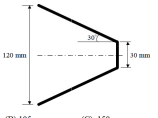
\includegraphics[width=0.5\linewidth]{figs/fig1.png}
    \caption{Figure-1}
    \label{fig:figs/fig1.png}
\end{figure}
     \begin{enumerate}
         \item 75
         \item 105
         \item 150
         \item 210
     \end{enumerate}
   
    \item For a classical (Wilson) model of determining economic order quantity (EOQ), the carrying and ordering costs are \( C_c \) and \( C_o \), respectively. For an annual demand \( D \), the minimum yearly total inventory cost is

     \hfill{(GATE 2019 PE)}\\
     \begin{enumerate}
         \item \(D C C_c\)
         \item \(\sqrt{1.5 D C C_c}\)
         \item \(\sqrt{2 D C C_c}\)
         \item \(\sqrt{3 D C C_o}\)
     \end{enumerate}
   
    \item A company has purchased an asset by investing Rs. 30,000. The useful life of the asset is 5 years and it has no salvage value at the end of its useful life. The depreciation cost (in Rs.) for the 2nd year using sum-of-years-digit (SYD) method is

     \hfill{(GATE 2019 PE)}\\
     \begin{enumerate}
         \item 10,000 
         \item  8,000
         \item 6,000 
         \item  4,000
     \end{enumerate}
   

    \item In a NC milling operation, the tool path is generated using absolute programming for the trajectory shown in the figure. The corresponding block of the NC program is

     \hfill{(GATE 2019 PE)}\\
     \begin{figure}[H]
         \centering
         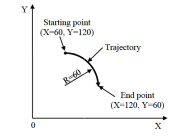
\includegraphics[width=0.5\linewidth]{figs/fig2.png}
         \caption{Figure-2}
         \label{fig:figs/fig2.png}
     \end{figure}
     \begin{enumerate}
         \item G02 X 120.0 Y 60.0 R 60.0
         \item G02 X 60.0 Y 120.0 R 60.0
         \item G03 X 60.0 Y 120.0 R 60.0
         \item G03 X 120.0 Y 60.0 R 60.0
         
     \end{enumerate}
  \item The SQC chart based on Binomial distribution is

     \hfill{(GATE 2019 PE)}\\
     \begin{enumerate}
         \item p chart
         \item c chart
         \item X chart
         \item R chart
     \end{enumerate}
    \item The capacity of a passenger airline is expressed in terms of 
    
    \hfill{(GATE 2019 PE)}\\
    \begin{enumerate}
        \item available seats
        \item available miles
        \item available sectors 
        \item available seat miles
    \end{enumerate}
     \item REL chart is used in  

    \hfill{(GATE 2019 PE)}\\
\begin{enumerate}
    \item  Quality management
    \item Inventory management
    \item Facility management 
    \item Human resource management
\end{enumerate}

    \item A metallic rod of diameter \(d_o\) is subjected to the tensile test. The engineering stress and the true stress at fracture are 800 MPa and 900 MPa, respectively. The ratio of the rod diameter at fracture \(d_f\) to the initial diameter \(d_o\) is  
    (round off to 2 decimal places)

    \hfill{(GATE 2019 PE)}\\

    \item A heat pump is to supply heat at the rate of 10 kW to a building to be maintained at 22~°C. The outside temperature is 2~°C. The minimum power (in kW) required to run the heat pump is  
    (round off to 2 decimal places)

    \hfill{(GATE 2019 PE)}\\

    \item One kilogram of air is compressed at constant temperature of 150~°C until its volume is halved. Considering gas constant \(R = 0.287 \text{ kJ/kg-K}\) for air, magnitude of heat rejected (in kJ) in the compression process is  
    (round off to 2 decimal places)

    \hfill{(GATE 2019 PE)}\\

    \item For the abrasive jet machining process, the ratio of abrasive volume to carrier gas volume is 0.25. Further, the ratio of abrasive density to carrier gas density is 25. The mass ratio of abrasive to the mixture of abrasive and carrier gas is  
    (round off to 2 decimal places)

    \hfill{(GATE 2019 PE)}\\

    \item In a typical turning tool life test, the following data are generated for tools A and B: 
    \begin{table}[h!]
\small
\setlength{\tabcolsep}{4pt}
\renewcommand{\arraystretch}{0.9}
\centering
\begin{tabular}{|c|c|c|p{1.8cm}|p{2.5cm}|c|}
\hline
Q. No & Type & Section & Key & Marks \\
\hline
1  & MCQ & GA & C         & 1 \\
\hline
2  & MCQ & GA & A         & 1 \\
\hline
3  & MCQ & GA & A         & 1 \\
\hline
4  & MCQ & GA & A         & 1 \\
\hline
5  & MCQ & GA & D         & 1 \\
\hline
6  & MCQ & GA & D         & \textbf{2} \\
\hline
7  & MCQ & GA & B         & 2 \\
\hline
8  & MCQ & GA & C         & 2 \\
\hline
9  & MCQ & GA & B         & 2 \\
\hline
10 & MCQ & GA & C         & 2 \\
\hline
11 & MCQ & EY & D         & 1 \\
\hline
12 & MCQ & EY & D         & 1 \\
\hline
13 & MCQ & EY & A; D      & 1 \\
\hline
14 & MCQ & EY & B         & 1 \\
\hline
15 & NAT & EY & 7.99 : 8.10 & 1 \\
\hline
16 & MCQ & EY & B         & 1 \\
\hline
17 & MCQ & EY & C         & 1 \\
\hline
18 & MCQ & EY & D         & 1 \\
\hline
19 & NAT & EY & 9.9 : 10.1  & 1 \\
\hline
20 & MCQ & EY & C         & 1 \\
\hline
21 & MCQ & EY & B         & 1 \\
\hline
22 & MCQ & EY & A         & 1 \\
\hline
23 & MCQ & EY & D         & 1 \\
\hline
24 & MCQ & EY & B         & 1 \\
\hline
25 & MCQ & EY & A         & 1 \\
\hline
26 & MCQ & EY & C         & 2 \\
\hline
27 & MCQ & EY & D         & 2 \\
\hline
28 & MCQ & EY & C         & 2 \\
\hline
29 & MCQ & EY & D         & 2 \\
\hline
30 & MCQ & EY & B         & 2 \\
\hline
31 & MCQ & EY & A         & 2 \\
\hline
32 & MCQ & EY & C         & 2 \\
\hline
33 & MCQ & EY & A         & 2 \\
\hline
34 & MCQ & EY & B         & 2 \\
\hline
35 & MCQ & EY & A         & 2 \\
\hline
36 & MCQ & EY & A         & 2 \\
\hline
37 & MCQ & EY & C         & 2 \\
\hline
38 & MCQ & EY & A         & 2 \\
\hline
39 & NAT & EY & 0.17 : 0.19 & 2 \\
\hline
40 & MCQ & EY & A         & 2 \\
\hline
41 & MCQ & EY & B         & 2 \\
\hline
42 & MCQ & EY & B         & 2 \\
\hline
43 & MCQ & EY & A         & 2 \\
\hline
44 & MCQ & EY & D         & 2 \\
\hline
45 & MCQ & EY & B         & 2 \\
\hline
46 & MCQ & EY & A         & 2 \\
\hline
47 & NAT & EY & 0.175 : 0.20 & 2 \\
\hline
48 & MCQ & EY & A         & 2 \\
\hline
49 & NAT & EY & 0.49 : 0.51  & 2 \\
\hline
50 & MCQ & EY & B         & 2 \\
\hline
51 & MCQ & EY & A         & 2 \\
\hline
52 & MCQ & EY & C         & 2 \\
\hline
53 & NAT & EY & 1660 : 1700 & 2 \\
\hline
54 & NAT & EY & 0.45 : 0.55 & 2 \\
\hline
55 & MCQ & EY & A         & 2 \\
\hline
\end{tabular}
\caption{GATE 2016 EY Answer Key Summary}
\end{table}

    Assuming the same tool life exponent for the tools, the value of constant in the Taylor's tool life equation (with cutting speed in m/min and tool life in min) is  
    (round off to 2 decimal places)

\hfill{(GATE 2019 PE)}\\
    \item The average proportion non-conforming of 20 samples each of size 100 items is 0.12. The upper control limit for the relevant chart is  
    (round off to 2 decimal places)

\hfill{(GATE 2019 PE)}\\
    \item For a process which is in a state of statistical control (within \(\pm 3 \sigma\)), estimated process standard deviation \(\sigma\) is 3 mm. The specification limits for the corresponding product are \(100 \pm 7\) mm. The capability ratio \(C_p\) is  
    (round off to 3 decimal places)

\hfill{(GATE 2019 PE)}\\
    \item In a work study experiment, normal time was recorded as 140 s with a rating of 100\%. Considering 2\% allowance, the standard time (in s) is  
    (round off to 1 decimal place)

\hfill{(GATE 2019 PE)}\\
    \item A warehouse has 1 loading dock and 3 persons for loading operations. The arrival rate of trucks follows Poisson distribution with a mean of 4 trucks/hour. The average loading time (by three persons together) per truck is exponentially distributed with a mean of 10 minutes. The charge of the trucks per hour and loading charges per person per hour are Rs. 20 and Rs. 6, respectively. The total cost (in Rs./hour) is  

    \hfill{(GATE 2019 PE)}\\


\subsection*{Q.26 -- Q.55 carry two marks each.}

\item If the Laplace transform of \(e^{at}\) is \(\frac{1}{s - a}\), the Laplace transform of \(t \cosh t\) is

  \hfill{(GATE 2019 PE)}\\
  \begin{enumerate}
      \item \(\frac{1 + s^2}{(s-1)^2}\)
      \item \(\frac{1}{s-0}\)
      \item  \(\frac{1 - s^2}{(2-s)^2}\)
      \item \(\frac{1+s^2}{1-s^2}\)
  \end{enumerate}

\item General solution of the Cauchy-Euler equation \(x^{2} \frac{d^{2}y}{dx^{2}} + 7x \frac{dy}{dx} + 16y = 0\) is

 \hfill{(GATE 2019 PE)}\\
 \begin{enumerate}
     \item \(y = c_1 x^{2} + c_2 x^{4}\)
     \item \(y = c_1 x^{2} + c_2 x^{4}\)
     \item \(y = (c_1 + c_2 \ln x) x^{4}\)
     \item \(y = c_1 x^{2} + 2x \ln x\)
 \end{enumerate}

\item A uniform cantilever beam ABC of length \(L\) is subjected to a point load \(P\) at point B and a concentrated moment \(M\) at point C (as shown in figure). Let \(E\) be Young's modulus and \(I\) the moment of inertia. Assuming Euler-Bernoulli beam theory, downward deflection at point C is

\hfill{(GATE 2019 PE)}\\
\begin{figure}[H]
    \centering
    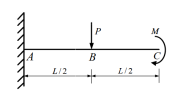
\includegraphics[width=0.5\linewidth]{figs/fig3.png}
    \caption{Figure-3}
    \label{fig:figs/fig3.png}
\end{figure}
\begin{enumerate}
    \item \(\frac{PL^{3}}{3EI} + \frac{ML^{2}}{2EI}\) 
    \item \(\frac{PL^{3}}{24EI} + \frac{ML^{2}}{2EI}\)
    \item \(\frac{PL^{3}}{48EI} + \frac{ML^{2}}{2EI}\) 
    \item \(\frac{5PL^{3}}{48EI} + \frac{ML^{2}}{2EI}\)
\end{enumerate}

\item Three Carnot engines \(E_1\), \(E_2\), and \(E_3\) operate between thermal reservoirs \(T_1 > T_2 > T_3\) as shown. The efficiency of engine \(E_3\) in terms of efficiencies \(\eta_1\) and \(\eta_2\) of engines \(E_1\) and \(E_2\), respectively, is

\hfill{(GATE 2019 PE)}\\
\begin{figure}[H]
    \centering
    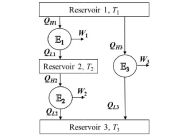
\includegraphics[width=0.5\linewidth]{figs/fig4.png}
    \caption{Figure-4}
    \label{fig:figs/fig4.png}
\end{figure}
\begin{enumerate}
    \item \(\eta_1 + \eta_2\)
    \item \(\eta_1 + \eta_2- \eta_1 \eta_2\)
    \item \(1-\eta_1-\eta_2\)
    \item  \(1 - \eta_1 \eta_2\)
\end{enumerate}

\item True centrifugal casting process in horizontal configuration is used to cast a metallic cylinder with outside diameter 0.275 m and inside diameter 0.250 m. If G-factor (ratio of centrifugal force to weight) is 65 and \(g=9.8\, m/s^2\), the minimum rotational speed (rpm) required is closest to

\hfill{(GATE 2019 PE)}\\
\begin{enumerate}
    \item 325
    \item 650
    \item 975
    \item 1300
\end{enumerate}

\item In a sine bar, let \(h\) denote slip gauge height and \(l\) distance between rollers. The relation between error in angular measurement \(d\theta\) and errors in slip gauge height \(dh\) and spacing \(dl\) is

\hfill{(GATE 2019 PE)}\\
\begin{enumerate}
    \item  \(d\theta = \sin \theta \left(\frac{dh}{h} - \frac{dl}{l}\right)\) 
    \item  \(d\theta = \cos \theta \left(\frac{dh}{h} - \frac{dl}{l}\right)\) 
    \item  \(d\theta = \tan \theta \left(\frac{dh}{h} - \frac{dl}{l}\right)\) 
    \item  \(d\theta = \cot \theta \left(\frac{dh}{h} - \frac{dl}{l}\right)\) 
    
\end{enumerate}

\item A 100 mm long cylindrical workpiece of diameter 50 mm is reduced to 25 mm diameter by extrusion. The flow curve has strength coefficient \(K=750\) MPa and strain hardening exponent 0.15. Assuming no friction or redundant work, the required ram pressure (MPa) is closest to

\hfill{(GATE 2019 PE)}\\
\begin{enumerate}
   
\item 164
\item 364
\item 428
\item 950
\end{enumerate}
\item An LPP is defined as:  
Minimize \(z=15x_1+12x_2\) subject to:  
\[
x_1 + 2x_2 \leq 3, \quad 2x_1 - 4x_2 \leq 5, \quad x_1,x_2 \geq 0
\]  
The objective function of the dual of this LLP is

\hfill{(GATE 2019 PE)}\\
\begin{enumerate}
    \item Maximize \(w = y_1 + y_2\)
    \item Maximize \(w = y_1 + 2 y_2\)
    \item Maximize \(w = 2y_1 - 4 y_2\)
    \item Maximize \(w = 3 y_1 + 5 y_2\)
\end{enumerate}

\item A 20 mm HSS drill with 118° point angle drills a 100 mm thick plate at 333.33 mm/s and 0.22 mm/rev feed. Assuming drill just touches plate surface at start, drilling time (s) is closest to

\hfill{(GATE 2019 PE)}\\
\begin{enumerate}
    \item 85
    \item 90
    \item 96
    \item 100
\end{enumerate}

\item An acceptance sampling plan with sample size \(n=80\), acceptance number \(c=2\) for a lot of 10,000 units, using Poisson distribution with rectification inspection and incoming lot quality \(p=0.03\), mean 2.4, has average outgoing quality (AOQ) closest to

\hfill{(GATE 2019 PE)}\\
\begin{enumerate}
    \item0.0011
    \item 0.0087
    \item 0.0170
    \item 0.0338
\end{enumerate}

\item Mean time to repair (MTTR) for repairable system is 30 min. When maintenance time increases from 20 to 40 min, net increase in maintainability is closest to

\hfill{(GATE 2019 PE)}\\
\begin{enumerate}
    \item 0.15
    \item 0.25
    \item0.45 
    \item 0.60
\end{enumerate}

\item A company invests Rs. 50,000 in assets: Rs. 30,000 initially, and Rs. 10,000 each at the end of 1st and 2nd years. Useful life is 10 years, no salvage value, interest rate 10\%, MARR 12\%. Annual capital recovery and return (CRR) in thousand Rs. is

\hfill{(GATE 2019 PE)}\\
\begin{enumerate}
    \item 8.38
    \item 7.06
    \item 5.74
    \item 3.10
\end{enumerate}

\item Man-hours required to manufacture the \(n\)th unit is given by \(T_n = T_1 n^{b}\), where \(b=-0.322\) at 80\% learning rate, manufacturing time for first unit is 80 man-hours. Total time to manufacture first 4 units (man-hours) is

\hfill{(GATE 2019 PE)}\\
\begin{enumerate}
    \item 322.11
    \item 251.35
    \item 103.76
    \item 51.19
\end{enumerate}

\item A firm with production target of 50,000 units/year has fixed and variable costs for locations P, Q, R, and S as:  
\[
\begin{array}{lll}
\text{Location} & \text{Fixed Cost (Rs.)} & \text{Variable Cost per unit (Rs.)} \\
P & 110,000 & 2 \\
Q & 95,000 & 2.5 \\
R & 80,000 & 3 \\
S & 75,000 & 3.5 \\
\end{array}
\]  
Most economical location is

\hfill{(GATE 2019 PE)}\\
\begin{enumerate}
    \item P
    \item Q
    \item R
    \item S
\end{enumerate}

\item Considering included angle of 60° using Best-Wire method, difference between effective diameter \(E\) and dimension under wire \(T\) for M10 x 1.0 mm is closest to

\hfill{(GATE 2019 PE)}\\
\begin{enumerate}
    \item 0.289
    \item 0.578
    \item 0.867
    \item 0.982
\end{enumerate}

\item If \(z\) is a complex variable with \(i = \sqrt{-1}\), length of minor axis of ellipse defined by \(|z-(1+i)| + |z-(9+i)| = 10\) is

\hfill{(GATE 2019 PE)}\\
(round off to between 5.9 to 6.1)

\item Numerical value of the definite integral \(\int_0^1 e^x dx\) using trapezoidal rule evaluated at points 0, 0.5, and 1 is

\hfill{(GATE 2019 PE)}\\
(round off to 3 decimal places)

\item A thin-walled cylindrical pressure vessel with inside diameter 300 mm and wall thickness 3 mm is subjected to internal gauge pressure of 1.5 MPa. Maximum shear stress (MPa) at inner surface is

\hfill{(GATE 2019 PE)}\\

\item A cam designed to achieve simple harmonic motion of a flat-faced follower rises 50 mm at 180° of cam rotation. If cam rotates at 100 rpm, speed of follower (mm/s) when cam rotates 45° from start is
\begin{figure}[H]
    \centering
    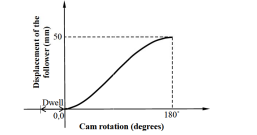
\includegraphics[width=0.5\linewidth]{figs/fig5.png}
    \caption{Figure-5}
    \label{fig:figs/fig5.png}
\end{figure}
\hfill{(GATE 2019 PE)}\\

\item An open tank of 2 x 2 x 2, $m^3$ is filled with layers of two fluids: 1 m of oil (SG 0.8) on top and 1 m of water. Density of water = 1000 kg/$m^3$, \(g=9.8\ m/s^2\). Force (N) exerted by fluids on one side wall is\\

\hfill{(GATE 2019 PE)}\\
\item During a storm, wind speed = 90 km/h. Window size = 1.2 x1.8m. Density of air = 1.2 kg/$m^3$. Force acting on window (N) is

\hfill{(GATE 2019 PE)}\\

\item Heat transfer efficiency in arc welding using current 250 A at 20 V is 90\%. Heat needed to melt material is 10 J/$mm^3$, weld cross-section 30$mm^3$, travel speed 5 mm/s, melting efficiency(\%) is

\hfill{(GATE 2019 PE)}\\

\item Sand casting process has mold constant 2 s/$mm^2$ and solidification exponent 2. If solidification time doubles for given volume, corresponding reduction in cast surface area (\%) is

\hfill{(GATE 2019 PE)}\\


\item During turning of material with shear strength 220 MPa, feed 0.2 mm/rev, depth 1 mm, rake angle 5°, chip thickness ratio 0.5, friction angle 49.2°, shear angle 25.4°, feed force (N) is
\begin{center}
\begin{tabular}{|p{1cm}|p{3cm}|p{1cm}|p{7cm}|}
\hline

\multicolumn{2}{|c|}{Process} & \multicolumn{2}{c|}{Application} \\
\hline
P & Extrusion & 1 & Producing complex parts with close tolerance \\
\hline
Q & Injection molding & 2 & Producing thermosetting plastic components \\
\hline
R & Blow molding & 3 & Producing long uniform sections \\
\hline
S & Compression molding & 4 & Producing hollow shapes \\
\hline
\end{tabular}
\end{center}
\hfill{(GATE 2019 PE)}\\

\item  A CO2 laser in continuous mode with power intensity $1x10^{x}$ W/$mm^2$, vaporization energy $5x10^{6}$J/$mm^3$, process efficiency 15\%, laser spot diameter 200 micrometers. Drilled depth (mm) after 2 sec is\\
\begin{figure}[H]
    \centering
    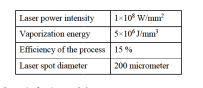
\includegraphics[width=0.5\linewidth]{figs/fig6.png}
    \caption{Table-4}
    \label{fig:figs/fig6.png}
\end{figure}
\hfill{(GATE 2019 PE)}\\
\item A Process with control limits \(\pm 3\sigma\), estimated \(\sigma=2\) mm, spec limits 120 \(\pm 8\) mm. When process mean shifts from 118 to 122 mm with same \(\sigma\), difference in process capability index \(C_{pk}\) is\\

\hfill{(GATE 2019 PE)}\\

\item A monitering system has seven component. Reliability of seven components  System reliability is\\
\begin{figure}[H]
    \centering
    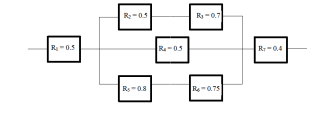
\includegraphics[width=0.5\linewidth]{figs/fig7.png}
    \caption{Figure-7}
    \label{fig:figs/fig7.png}
\end{figure}

\hfill{(GATE 2019 PE)}\\

\item PERT project network consists of 5 activities A to E. The time estimates of these activities follow Beta-distribution. The predeceesor-succesor(P-S)relatoinship betweenthe nodes and the time estimates of activitiesare given in table.
\hfill{(GATE 2019 PE)}\\
\begin{figure}[H]
    \centering
    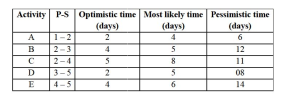
\includegraphics[width=1\linewidth]{figs/fig8.png}\\
    The variance (in days) of the critical path is,
    \caption{Table-4}
    \label{fig:figs/fig8.png}
\end{figure}
\item Sales data of a product for 5 years are
\begin{tabular}[12pt]{ |c| c| c| c| c| c| }
    \hline
   Q.No. & Session & Que.Type & Sec. Name & Key & Marks \\
    \hline
    46 & 4 & NAT & AE & 149.0 to 151.0 & 2\\
    \hline
    47 & 4 & NAT & AE & 1712.0 to 1719.0 & 2\\
    \hline
    48 & 4 & NAT & AE & 91 to 93 & 2\\
    \hline
    49 & 4 & NAT & AE & 87 to 89 & 2\\
    \hline
    50 & 4 & NAT & AE & 27.0 to 27.2 & 2\\
    \hline
    51 & 4 & NAT & AE & 1.43 to 1.45 & 2\\
    \hline
    52 & 4 & NAT & AE & 0.61 to 0.63 & 2\\
    \hline
    53 & 4 & NAT & AE & 3.74 to 3.76 & 2\\
    \hline
    54 & 4 & NAT & AE & 62.95 to 63.08 & 2\\
    \hline
    55 & 4 & NAT & AE & 57.10 to 60.00 & 2\\
    \hline
\end{tabular}


Assume the forecast for the year 2014 as 260 units. Using an exponential smoothig method with smoothing constant $\alpha$ = 0.5, the sales forecast for year 2019, is
\hfill{(GATE 2019 PE)}\\

\item Layout for AGV system shown. The loading time is 0.5 minutes and the unloading time is also 0.5 minutes. All distances are in meters.
\begin{figure}[H]
    \centering
    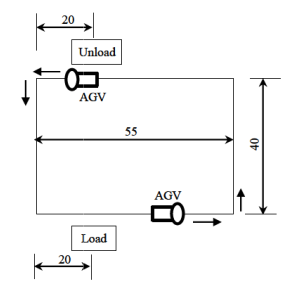
\includegraphics[width=0.5\linewidth]{figs/fig9.png}
    \caption{Figure-9}
    \label{fig:figs/fig9.png}
\end{figure}

Considering the vehicle velocity of 50 m/min, availablity of 0.95 and traffic factor fo 0.9, the number of vehicles required to satisfy a demand of 50 delhivery/hour is

\hfill{(GATE 2019 PE)}\\
\end{enumerate}
\end{document}